\documentclass{book}
\usepackage[a4paper,top=2.5cm,bottom=2.5cm,left=2.5cm,right=2.5cm]{geometry}
\usepackage{makeidx}
\usepackage{natbib}
\usepackage{graphicx}
\usepackage{multicol}
\usepackage{float}
\usepackage{listings}
\usepackage{color}
\usepackage{ifthen}
\usepackage[table]{xcolor}
\usepackage{textcomp}
\usepackage{alltt}
\usepackage{ifpdf}
\ifpdf
\usepackage[pdftex,
            pagebackref=true,
            colorlinks=true,
            linkcolor=blue,
            unicode
           ]{hyperref}
\else
\usepackage[ps2pdf,
            pagebackref=true,
            colorlinks=true,
            linkcolor=blue,
            unicode
           ]{hyperref}
\usepackage{pspicture}
\fi
\usepackage[utf8]{inputenc}
\usepackage{polski}
\usepackage[T1]{fontenc}

\usepackage{mathptmx}
\usepackage[scaled=.90]{helvet}
\usepackage{courier}
\usepackage{sectsty}
\usepackage{amssymb}
\usepackage[titles]{tocloft}
\usepackage{doxygen}
\lstset{language=C++,inputencoding=utf8,basicstyle=\footnotesize,breaklines=true,breakatwhitespace=true,tabsize=8,numbers=left }
\makeindex
\setcounter{tocdepth}{3}
\renewcommand{\footrulewidth}{0.4pt}
\renewcommand{\familydefault}{\sfdefault}
\hfuzz=15pt
\setlength{\emergencystretch}{15pt}
\hbadness=750
\tolerance=750
\begin{document}
\hypersetup{pageanchor=false,citecolor=blue}
\begin{titlepage}
\vspace*{7cm}
\begin{center}
{\Large Lab 2 P\-A\-M\-S\-I \\[1ex]\large 0.\-1 }\\
\vspace*{1cm}
{\large Wygenerowano przez Doxygen 1.8.1.2}\\
\vspace*{0.5cm}
{\small Pn, 10 mar 2014 00:11:31}\\
\end{center}
\end{titlepage}
\clearemptydoublepage
\pagenumbering{roman}
\tableofcontents
\clearemptydoublepage
\pagenumbering{arabic}
\hypersetup{pageanchor=true,citecolor=blue}
\chapter{Dokumentacja zadania P\-A\-M\-S\-I L\-A\-B 2}
\label{index}\hypertarget{index}{}\begin{DoxyAuthor}{Author}
Justyna Klijewska 
\end{DoxyAuthor}
\begin{DoxyDate}{Date}
28.\-05.\-2014 
\end{DoxyDate}
\begin{DoxyVersion}{Version}
0.\-1 
\end{DoxyVersion}

\chapter{Indeks klas}
\section{Lista klas}
Tutaj znajdują się klasy, struktury, unie i interfejsy wraz z ich krótkimi opisami\-:\begin{DoxyCompactList}
\item\contentsline{section}{\hyperlink{class_tablica}{Tablica} }{\pageref{class_tablica}}{}
\item\contentsline{section}{\hyperlink{class_zegar}{Zegar} }{\pageref{class_zegar}}{}
\end{DoxyCompactList}

\chapter{Indeks plików}
\section{File List}
Here is a list of all files with brief descriptions\-:\begin{DoxyCompactList}
\item\contentsline{section}{C\-:/\-Users/\-Klijek/\-Documents/\-Git\-Hub/\-Pamis02/\-L\-A\-B8/prj/\hyperlink{graf_8cpp}{graf.\-cpp} }{\pageref{graf_8cpp}}{}
\item\contentsline{section}{C\-:/\-Users/\-Klijek/\-Documents/\-Git\-Hub/\-Pamis02/\-L\-A\-B8/prj/\hyperlink{graf_8hpp}{graf.\-hpp} }{\pageref{graf_8hpp}}{}
\item\contentsline{section}{C\-:/\-Users/\-Klijek/\-Documents/\-Git\-Hub/\-Pamis02/\-L\-A\-B8/prj/\hyperlink{main_8cpp}{main.\-cpp} }{\pageref{main_8cpp}}{}
\end{DoxyCompactList}

\chapter{Dokumentacja klas}
\hypertarget{class_tablica}{\section{Dokumentacja klasy Tablica}
\label{class_tablica}\index{Tablica@{Tablica}}
}


{\ttfamily \#include $<$tablica.\-hpp$>$}

\subsection*{Metody publiczne}
\begin{DoxyCompactItemize}
\item 
\hyperlink{class_tablica_a5f484e7b0478e1ff9b62e894f9d7b28d}{Tablica} ()
\item 
void \hyperlink{class_tablica_ae1af903a66629cd0d522eb9f2fd13116}{Push} (double ele)
\item 
double \hyperlink{class_tablica_a6153881ffda3f5361c2d664622a4eff4}{Pop} ()
\item 
double \hyperlink{class_tablica_a899c8e69cb97bd027c1c05140cd304ec}{Pop\-\_\-\-Back} ()
\item 
int \hyperlink{class_tablica_a8598f952095406441bfd2d20e76f175c}{Size} ()
\item 
void \hyperlink{class_tablica_a08b59415756d2dc7da781124809d8eb4}{Isempty} ()
\item 
void \hyperlink{class_tablica_a06c551a7e0220dde2f29cce06fb96209}{Show\-\_\-\-Tab} ()
\item 
\hyperlink{class_tablica}{Tablica} \hyperlink{class_tablica_a15c072e7160bfbdbc5d103cf0ebd6e76}{operator+} (\hyperlink{class_tablica}{Tablica} \&T2)
\item 
\hyperlink{class_tablica}{Tablica} \hyperlink{class_tablica_acabfd453d919950051b8a9cf4aac642e}{operator$\ast$} (double M)
\item 
\hyperlink{class_tablica}{Tablica} \hyperlink{class_tablica_a53bd7c9853f01a78ba2aff61ece4ccbf}{operator=} (\hyperlink{class_tablica}{Tablica} \&T2)
\item 
\hyperlink{class_tablica}{Tablica} \hyperlink{class_tablica_ae5d9fdf31df882eae683abc89fec01ad}{operator==} (\hyperlink{class_tablica}{Tablica} \&T2)
\end{DoxyCompactItemize}
\subsection*{Przyjaciele}
\begin{DoxyCompactItemize}
\item 
void \hyperlink{class_tablica_a17e08e601d94bc6fce93c91bd574e717}{Quick\-\_\-\-Sort} (\hyperlink{class_tablica}{Tablica} \&T, int left, int right)
\item 
void \hyperlink{class_tablica_a7ac406a30a3a7a46d498f05bb173809c}{Heap\-\_\-\-Sort} (\hyperlink{class_tablica}{Tablica} \&T)
\item 
void \hyperlink{class_tablica_ae6edf270c00af312bbafffc1955450cc}{Merge} (\hyperlink{class_tablica}{Tablica} \&T, int left, int cent, int right)
\end{DoxyCompactItemize}


\subsection{Opis szczegółowy}


Definicja w linii 14 pliku tablica.\-hpp.



\subsection{Dokumentacja konstruktora i destruktora}
\hypertarget{class_tablica_a5f484e7b0478e1ff9b62e894f9d7b28d}{\index{Tablica@{Tablica}!Tablica@{Tablica}}
\index{Tablica@{Tablica}!Tablica@{Tablica}}
\subsubsection[{Tablica}]{\setlength{\rightskip}{0pt plus 5cm}Tablica\-::\-Tablica (
\begin{DoxyParamCaption}
{}
\end{DoxyParamCaption}
)\hspace{0.3cm}{\ttfamily [inline]}}}\label{class_tablica_a5f484e7b0478e1ff9b62e894f9d7b28d}


Definicja w linii 20 pliku tablica.\-hpp.



\subsection{Dokumentacja funkcji składowych}
\hypertarget{class_tablica_a08b59415756d2dc7da781124809d8eb4}{\index{Tablica@{Tablica}!Isempty@{Isempty}}
\index{Isempty@{Isempty}!Tablica@{Tablica}}
\subsubsection[{Isempty}]{\setlength{\rightskip}{0pt plus 5cm}void Tablica\-::\-Isempty (
\begin{DoxyParamCaption}
{}
\end{DoxyParamCaption}
)}}\label{class_tablica_a08b59415756d2dc7da781124809d8eb4}


Definicja w linii 98 pliku tablica.\-cpp.



Oto graf wywoływań tej funkcji\-:


\hypertarget{class_tablica_acabfd453d919950051b8a9cf4aac642e}{\index{Tablica@{Tablica}!operator$\ast$@{operator$\ast$}}
\index{operator$\ast$@{operator$\ast$}!Tablica@{Tablica}}
\subsubsection[{operator$\ast$}]{\setlength{\rightskip}{0pt plus 5cm}{\bf Tablica} Tablica\-::operator$\ast$ (
\begin{DoxyParamCaption}
\item[{double}]{M}
\end{DoxyParamCaption}
)}}\label{class_tablica_acabfd453d919950051b8a9cf4aac642e}


Definicja w linii 264 pliku tablica.\-cpp.

\hypertarget{class_tablica_a15c072e7160bfbdbc5d103cf0ebd6e76}{\index{Tablica@{Tablica}!operator+@{operator+}}
\index{operator+@{operator+}!Tablica@{Tablica}}
\subsubsection[{operator+}]{\setlength{\rightskip}{0pt plus 5cm}{\bf Tablica} Tablica\-::operator+ (
\begin{DoxyParamCaption}
\item[{{\bf Tablica} \&}]{T2}
\end{DoxyParamCaption}
)}}\label{class_tablica_a15c072e7160bfbdbc5d103cf0ebd6e76}


Definicja w linii 194 pliku tablica.\-cpp.

\hypertarget{class_tablica_a53bd7c9853f01a78ba2aff61ece4ccbf}{\index{Tablica@{Tablica}!operator=@{operator=}}
\index{operator=@{operator=}!Tablica@{Tablica}}
\subsubsection[{operator=}]{\setlength{\rightskip}{0pt plus 5cm}{\bf Tablica} Tablica\-::operator= (
\begin{DoxyParamCaption}
\item[{{\bf Tablica} \&}]{T2}
\end{DoxyParamCaption}
)}}\label{class_tablica_a53bd7c9853f01a78ba2aff61ece4ccbf}


Definicja w linii 209 pliku tablica.\-cpp.

\hypertarget{class_tablica_ae5d9fdf31df882eae683abc89fec01ad}{\index{Tablica@{Tablica}!operator==@{operator==}}
\index{operator==@{operator==}!Tablica@{Tablica}}
\subsubsection[{operator==}]{\setlength{\rightskip}{0pt plus 5cm}{\bf Tablica} Tablica\-::operator== (
\begin{DoxyParamCaption}
\item[{{\bf Tablica} \&}]{T2}
\end{DoxyParamCaption}
)}}\label{class_tablica_ae5d9fdf31df882eae683abc89fec01ad}


Definicja w linii 220 pliku tablica.\-cpp.

\hypertarget{class_tablica_a6153881ffda3f5361c2d664622a4eff4}{\index{Tablica@{Tablica}!Pop@{Pop}}
\index{Pop@{Pop}!Tablica@{Tablica}}
\subsubsection[{Pop}]{\setlength{\rightskip}{0pt plus 5cm}double Tablica\-::\-Pop (
\begin{DoxyParamCaption}
{}
\end{DoxyParamCaption}
)}}\label{class_tablica_a6153881ffda3f5361c2d664622a4eff4}


Definicja w linii 33 pliku tablica.\-cpp.



Oto graf wywoływań tej funkcji\-:


\hypertarget{class_tablica_a899c8e69cb97bd027c1c05140cd304ec}{\index{Tablica@{Tablica}!Pop\-\_\-\-Back@{Pop\-\_\-\-Back}}
\index{Pop\-\_\-\-Back@{Pop\-\_\-\-Back}!Tablica@{Tablica}}
\subsubsection[{Pop\-\_\-\-Back}]{\setlength{\rightskip}{0pt plus 5cm}double Tablica\-::\-Pop\-\_\-\-Back (
\begin{DoxyParamCaption}
{}
\end{DoxyParamCaption}
)}}\label{class_tablica_a899c8e69cb97bd027c1c05140cd304ec}


Definicja w linii 59 pliku tablica.\-cpp.



Oto graf wywoływań tej funkcji\-:


\hypertarget{class_tablica_ae1af903a66629cd0d522eb9f2fd13116}{\index{Tablica@{Tablica}!Push@{Push}}
\index{Push@{Push}!Tablica@{Tablica}}
\subsubsection[{Push}]{\setlength{\rightskip}{0pt plus 5cm}void Tablica\-::\-Push (
\begin{DoxyParamCaption}
\item[{double}]{ele}
\end{DoxyParamCaption}
)}}\label{class_tablica_ae1af903a66629cd0d522eb9f2fd13116}


Definicja w linii 17 pliku tablica.\-cpp.



Oto graf wywoływań tej funkcji\-:


\hypertarget{class_tablica_a06c551a7e0220dde2f29cce06fb96209}{\index{Tablica@{Tablica}!Show\-\_\-\-Tab@{Show\-\_\-\-Tab}}
\index{Show\-\_\-\-Tab@{Show\-\_\-\-Tab}!Tablica@{Tablica}}
\subsubsection[{Show\-\_\-\-Tab}]{\setlength{\rightskip}{0pt plus 5cm}void Tablica\-::\-Show\-\_\-\-Tab (
\begin{DoxyParamCaption}
{}
\end{DoxyParamCaption}
)}}\label{class_tablica_a06c551a7e0220dde2f29cce06fb96209}


Definicja w linii 167 pliku tablica.\-cpp.



Oto graf wywoływań tej funkcji\-:


\hypertarget{class_tablica_a8598f952095406441bfd2d20e76f175c}{\index{Tablica@{Tablica}!Size@{Size}}
\index{Size@{Size}!Tablica@{Tablica}}
\subsubsection[{Size}]{\setlength{\rightskip}{0pt plus 5cm}int Tablica\-::\-Size (
\begin{DoxyParamCaption}
{}
\end{DoxyParamCaption}
)}}\label{class_tablica_a8598f952095406441bfd2d20e76f175c}


Definicja w linii 86 pliku tablica.\-cpp.



Oto graf wywoływań tej funkcji\-:




\subsection{Dokumentacja przyjaciół i funkcji związanych}
\hypertarget{class_tablica_a7ac406a30a3a7a46d498f05bb173809c}{\index{Tablica@{Tablica}!Heap\-\_\-\-Sort@{Heap\-\_\-\-Sort}}
\index{Heap\-\_\-\-Sort@{Heap\-\_\-\-Sort}!Tablica@{Tablica}}
\subsubsection[{Heap\-\_\-\-Sort}]{\setlength{\rightskip}{0pt plus 5cm}void Heap\-\_\-\-Sort (
\begin{DoxyParamCaption}
\item[{{\bf Tablica} \&}]{T}
\end{DoxyParamCaption}
)\hspace{0.3cm}{\ttfamily [friend]}}}\label{class_tablica_a7ac406a30a3a7a46d498f05bb173809c}


Definicja w linii 34 pliku sort.\-cpp.

\hypertarget{class_tablica_ae6edf270c00af312bbafffc1955450cc}{\index{Tablica@{Tablica}!Merge@{Merge}}
\index{Merge@{Merge}!Tablica@{Tablica}}
\subsubsection[{Merge}]{\setlength{\rightskip}{0pt plus 5cm}void Merge (
\begin{DoxyParamCaption}
\item[{{\bf Tablica} \&}]{T, }
\item[{int}]{left, }
\item[{int}]{cent, }
\item[{int}]{right}
\end{DoxyParamCaption}
)\hspace{0.3cm}{\ttfamily [friend]}}}\label{class_tablica_ae6edf270c00af312bbafffc1955450cc}


Definicja w linii 79 pliku sort.\-cpp.

\hypertarget{class_tablica_a17e08e601d94bc6fce93c91bd574e717}{\index{Tablica@{Tablica}!Quick\-\_\-\-Sort@{Quick\-\_\-\-Sort}}
\index{Quick\-\_\-\-Sort@{Quick\-\_\-\-Sort}!Tablica@{Tablica}}
\subsubsection[{Quick\-\_\-\-Sort}]{\setlength{\rightskip}{0pt plus 5cm}void Quick\-\_\-\-Sort (
\begin{DoxyParamCaption}
\item[{{\bf Tablica} \&}]{T, }
\item[{int}]{left, }
\item[{int}]{right}
\end{DoxyParamCaption}
)\hspace{0.3cm}{\ttfamily [friend]}}}\label{class_tablica_a17e08e601d94bc6fce93c91bd574e717}


Definicja w linii 3 pliku sort.\-cpp.



Dokumentacja dla tej klasy została wygenerowana z plików\-:\begin{DoxyCompactItemize}
\item 
C\-:/\-Users/\-Klijek/\-Desktop/\-L\-A\-B4/prj/\hyperlink{tablica_8hpp}{tablica.\-hpp}\item 
C\-:/\-Users/\-Klijek/\-Desktop/\-L\-A\-B4/prj/\hyperlink{tablica_8cpp}{tablica.\-cpp}\end{DoxyCompactItemize}

\hypertarget{class_zegar}{\section{Dokumentacja klasy Zegar}
\label{class_zegar}\index{Zegar@{Zegar}}
}


{\ttfamily \#include $<$zegar.\-hpp$>$}

\subsection*{Metody publiczne}
\begin{DoxyCompactItemize}
\item 
void \hyperlink{class_zegar_af747dc3a9d58207618ec877990900b80}{Start} ()
\item 
void \hyperlink{class_zegar_a8a88ddd1aa0768bfbe37217e32a01da0}{Koniec} ()
\item 
void \hyperlink{class_zegar_a659d8f393442747d17aba3a5f6533c29}{Wynik} ()
\end{DoxyCompactItemize}


\subsection{Opis szczegółowy}


Definicja w linii 16 pliku zegar.\-hpp.



\subsection{Dokumentacja funkcji składowych}
\hypertarget{class_zegar_a8a88ddd1aa0768bfbe37217e32a01da0}{\index{Zegar@{Zegar}!Koniec@{Koniec}}
\index{Koniec@{Koniec}!Zegar@{Zegar}}
\subsubsection[{Koniec}]{\setlength{\rightskip}{0pt plus 5cm}void Zegar\-::\-Koniec (
\begin{DoxyParamCaption}
{}
\end{DoxyParamCaption}
)}}\label{class_zegar_a8a88ddd1aa0768bfbe37217e32a01da0}


Definicja w linii 20 pliku zegar.\-cpp.



Oto graf wywoływań tej funkcji\-:


\hypertarget{class_zegar_af747dc3a9d58207618ec877990900b80}{\index{Zegar@{Zegar}!Start@{Start}}
\index{Start@{Start}!Zegar@{Zegar}}
\subsubsection[{Start}]{\setlength{\rightskip}{0pt plus 5cm}void Zegar\-::\-Start (
\begin{DoxyParamCaption}
{}
\end{DoxyParamCaption}
)}}\label{class_zegar_af747dc3a9d58207618ec877990900b80}


Definicja w linii 9 pliku zegar.\-cpp.



Oto graf wywoływań tej funkcji\-:


\hypertarget{class_zegar_a659d8f393442747d17aba3a5f6533c29}{\index{Zegar@{Zegar}!Wynik@{Wynik}}
\index{Wynik@{Wynik}!Zegar@{Zegar}}
\subsubsection[{Wynik}]{\setlength{\rightskip}{0pt plus 5cm}void Zegar\-::\-Wynik (
\begin{DoxyParamCaption}
{}
\end{DoxyParamCaption}
)}}\label{class_zegar_a659d8f393442747d17aba3a5f6533c29}


Definicja w linii 36 pliku zegar.\-cpp.



Oto graf wywoływań tej funkcji\-:




Dokumentacja dla tej klasy została wygenerowana z plików\-:\begin{DoxyCompactItemize}
\item 
C\-:/\-Users/\-Klijek/\-Desktop/\-L\-A\-B4/prj/\hyperlink{zegar_8hpp}{zegar.\-hpp}\item 
C\-:/\-Users/\-Klijek/\-Desktop/\-L\-A\-B4/prj/\hyperlink{zegar_8cpp}{zegar.\-cpp}\end{DoxyCompactItemize}

\chapter{Dokumentacja plików}
\hypertarget{main_8cpp}{\section{Dokumentacja pliku C\-:/\-Users/\-Klijek/\-Desktop/\-L\-A\-B6/prj/main.cpp}
\label{main_8cpp}\index{C\-:/\-Users/\-Klijek/\-Desktop/\-L\-A\-B6/prj/main.\-cpp@{C\-:/\-Users/\-Klijek/\-Desktop/\-L\-A\-B6/prj/main.\-cpp}}
}
{\ttfamily \#include $<$iostream$>$}\\*
{\ttfamily \#include $<$string$>$}\\*
{\ttfamily \#include \char`\"{}tab\-Aso.\-hpp\char`\"{}}\\*
Wykres zależności załączania dla main.\-cpp\-:
\subsection*{Funkcje}
\begin{DoxyCompactItemize}
\item 
int \hyperlink{main_8cpp_ae66f6b31b5ad750f1fe042a706a4e3d4}{main} ()
\end{DoxyCompactItemize}


\subsection{Dokumentacja funkcji}
\hypertarget{main_8cpp_ae66f6b31b5ad750f1fe042a706a4e3d4}{\index{main.\-cpp@{main.\-cpp}!main@{main}}
\index{main@{main}!main.cpp@{main.\-cpp}}
\subsubsection[{main}]{\setlength{\rightskip}{0pt plus 5cm}int main (
\begin{DoxyParamCaption}
{}
\end{DoxyParamCaption}
)}}\label{main_8cpp_ae66f6b31b5ad750f1fe042a706a4e3d4}
Main

Przykladowe operacje na tablicy alokacyjnej. Wyswietlanie operacji.

Definicja w linii 13 pliku main.\-cpp.



Oto graf wywołań dla tej funkcji\-:



\hypertarget{operacje_8cpp}{\section{Dokumentacja pliku prj/operacje.cpp}
\label{operacje_8cpp}\index{prj/operacje.\-cpp@{prj/operacje.\-cpp}}
}
{\ttfamily \#include \char`\"{}operacje.\-hpp\char`\"{}}\\*
Wykres zależności załączania dla operacje.\-cpp\-:
\nopagebreak
\begin{figure}[H]
\begin{center}
\leavevmode
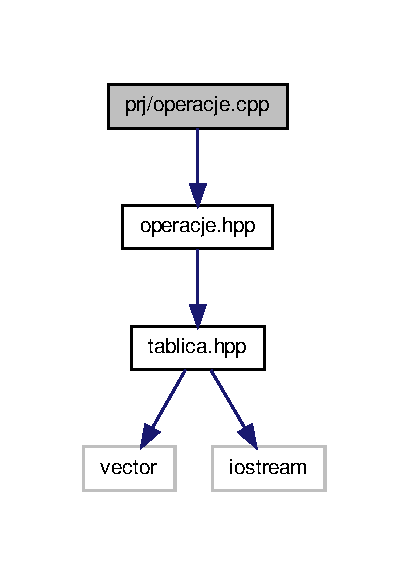
\includegraphics[width=196pt]{operacje_8cpp__incl}
\end{center}
\end{figure}
\subsection*{Funkcje}
\begin{DoxyCompactItemize}
\item 
void \hyperlink{operacje_8cpp_a0e1dcf6202da97bb49029fd97c1dc6a9}{Zamien\-Ele} (\hyperlink{class_tablica}{Tablica} \&T, int m1, int m2)
\item 
void \hyperlink{operacje_8cpp_a0933bc7e6ecc1138cde73ad221d3a6a6}{Odwroc\-Tab} (\hyperlink{class_tablica}{Tablica} \&T)
\item 
void \hyperlink{operacje_8cpp_a622767484b449600cf6446da085c561e}{Dodaj\-Ele} (\hyperlink{class_tablica}{Tablica} \&T, double ele)
\item 
void \hyperlink{operacje_8cpp_afcebfcc0c075278505a19b1c9afff30d}{Dodaj\-Ele} (\hyperlink{class_tablica}{Tablica} \&T1, \hyperlink{class_tablica}{Tablica} \&T2, double ele)
\end{DoxyCompactItemize}


\subsection{Dokumentacja funkcji}
\hypertarget{operacje_8cpp_a622767484b449600cf6446da085c561e}{\index{operacje.\-cpp@{operacje.\-cpp}!Dodaj\-Ele@{Dodaj\-Ele}}
\index{Dodaj\-Ele@{Dodaj\-Ele}!operacje.cpp@{operacje.\-cpp}}
\subsubsection[{Dodaj\-Ele}]{\setlength{\rightskip}{0pt plus 5cm}void Dodaj\-Ele (
\begin{DoxyParamCaption}
\item[{{\bf Tablica} \&}]{T, }
\item[{double}]{ele}
\end{DoxyParamCaption}
)}}\label{operacje_8cpp_a622767484b449600cf6446da085c561e}


Definicja w linii 14 pliku operacje.\-cpp.



Oto graf wywołań dla tej funkcji\-:
\nopagebreak
\begin{figure}[H]
\begin{center}
\leavevmode
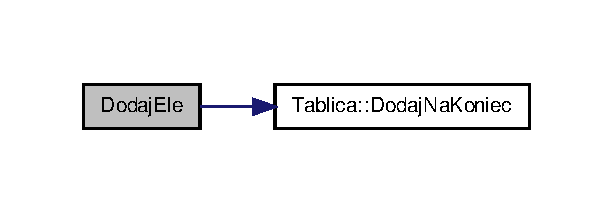
\includegraphics[width=294pt]{operacje_8cpp_a622767484b449600cf6446da085c561e_cgraph}
\end{center}
\end{figure}




Oto graf wywoływań tej funkcji\-:
\nopagebreak
\begin{figure}[H]
\begin{center}
\leavevmode
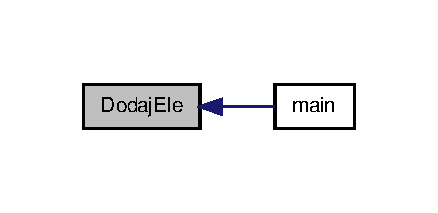
\includegraphics[width=210pt]{operacje_8cpp_a622767484b449600cf6446da085c561e_icgraph}
\end{center}
\end{figure}


\hypertarget{operacje_8cpp_afcebfcc0c075278505a19b1c9afff30d}{\index{operacje.\-cpp@{operacje.\-cpp}!Dodaj\-Ele@{Dodaj\-Ele}}
\index{Dodaj\-Ele@{Dodaj\-Ele}!operacje.cpp@{operacje.\-cpp}}
\subsubsection[{Dodaj\-Ele}]{\setlength{\rightskip}{0pt plus 5cm}void Dodaj\-Ele (
\begin{DoxyParamCaption}
\item[{{\bf Tablica} \&}]{T1, }
\item[{{\bf Tablica} \&}]{T2, }
\item[{double}]{ele}
\end{DoxyParamCaption}
)}}\label{operacje_8cpp_afcebfcc0c075278505a19b1c9afff30d}


Definicja w linii 20 pliku operacje.\-cpp.



Oto graf wywołań dla tej funkcji\-:
\nopagebreak
\begin{figure}[H]
\begin{center}
\leavevmode
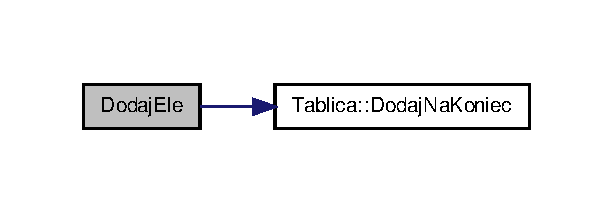
\includegraphics[width=294pt]{operacje_8cpp_afcebfcc0c075278505a19b1c9afff30d_cgraph}
\end{center}
\end{figure}


\hypertarget{operacje_8cpp_a0933bc7e6ecc1138cde73ad221d3a6a6}{\index{operacje.\-cpp@{operacje.\-cpp}!Odwroc\-Tab@{Odwroc\-Tab}}
\index{Odwroc\-Tab@{Odwroc\-Tab}!operacje.cpp@{operacje.\-cpp}}
\subsubsection[{Odwroc\-Tab}]{\setlength{\rightskip}{0pt plus 5cm}void Odwroc\-Tab (
\begin{DoxyParamCaption}
\item[{{\bf Tablica} \&}]{T}
\end{DoxyParamCaption}
)}}\label{operacje_8cpp_a0933bc7e6ecc1138cde73ad221d3a6a6}


Definicja w linii 9 pliku operacje.\-cpp.



Oto graf wywołań dla tej funkcji\-:
\nopagebreak
\begin{figure}[H]
\begin{center}
\leavevmode
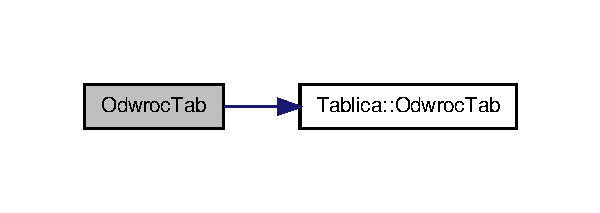
\includegraphics[width=288pt]{operacje_8cpp_a0933bc7e6ecc1138cde73ad221d3a6a6_cgraph}
\end{center}
\end{figure}




Oto graf wywoływań tej funkcji\-:
\nopagebreak
\begin{figure}[H]
\begin{center}
\leavevmode
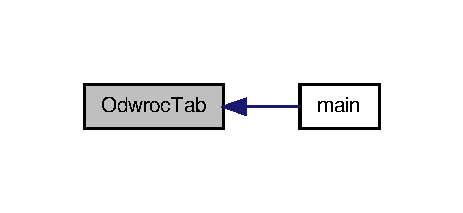
\includegraphics[width=222pt]{operacje_8cpp_a0933bc7e6ecc1138cde73ad221d3a6a6_icgraph}
\end{center}
\end{figure}


\hypertarget{operacje_8cpp_a0e1dcf6202da97bb49029fd97c1dc6a9}{\index{operacje.\-cpp@{operacje.\-cpp}!Zamien\-Ele@{Zamien\-Ele}}
\index{Zamien\-Ele@{Zamien\-Ele}!operacje.cpp@{operacje.\-cpp}}
\subsubsection[{Zamien\-Ele}]{\setlength{\rightskip}{0pt plus 5cm}void Zamien\-Ele (
\begin{DoxyParamCaption}
\item[{{\bf Tablica} \&}]{T, }
\item[{int}]{m1, }
\item[{int}]{m2}
\end{DoxyParamCaption}
)}}\label{operacje_8cpp_a0e1dcf6202da97bb49029fd97c1dc6a9}


Definicja w linii 4 pliku operacje.\-cpp.



Oto graf wywołań dla tej funkcji\-:
\nopagebreak
\begin{figure}[H]
\begin{center}
\leavevmode
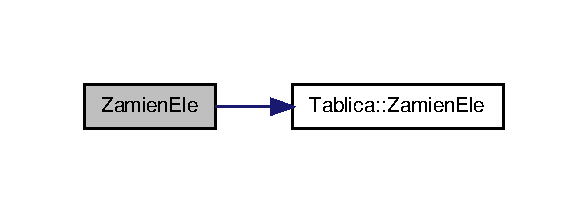
\includegraphics[width=282pt]{operacje_8cpp_a0e1dcf6202da97bb49029fd97c1dc6a9_cgraph}
\end{center}
\end{figure}




Oto graf wywoływań tej funkcji\-:
\nopagebreak
\begin{figure}[H]
\begin{center}
\leavevmode
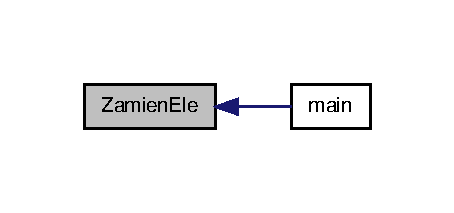
\includegraphics[width=218pt]{operacje_8cpp_a0e1dcf6202da97bb49029fd97c1dc6a9_icgraph}
\end{center}
\end{figure}



\hypertarget{operacje_8hpp}{\section{Dokumentacja pliku prj/operacje.hpp}
\label{operacje_8hpp}\index{prj/operacje.\-hpp@{prj/operacje.\-hpp}}
}


Definicja funkcji Zamien\-Ele.  


{\ttfamily \#include \char`\"{}tablica.\-hpp\char`\"{}}\\*
Wykres zależności załączania dla operacje.\-hpp\-:
\nopagebreak
\begin{figure}[H]
\begin{center}
\leavevmode
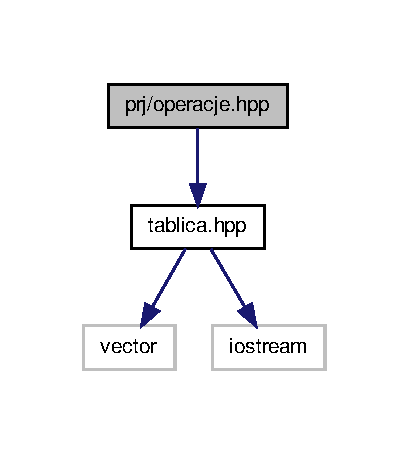
\includegraphics[width=196pt]{operacje_8hpp__incl}
\end{center}
\end{figure}
Ten wykres pokazuje, które pliki bezpośrednio lub pośrednio załączają ten plik\-:
\nopagebreak
\begin{figure}[H]
\begin{center}
\leavevmode
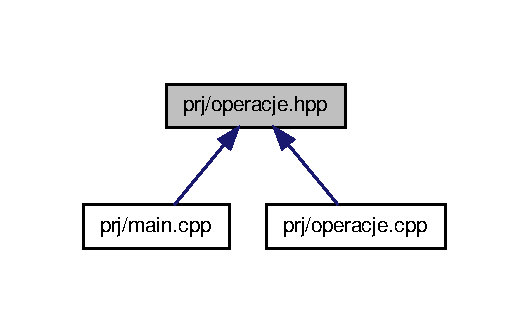
\includegraphics[width=254pt]{operacje_8hpp__dep__incl}
\end{center}
\end{figure}
\subsection*{Funkcje}
\begin{DoxyCompactItemize}
\item 
void \hyperlink{operacje_8hpp_a0e1dcf6202da97bb49029fd97c1dc6a9}{Zamien\-Ele} (\hyperlink{class_tablica}{Tablica} \&T, int m1, int m2)
\item 
void \hyperlink{operacje_8hpp_a0933bc7e6ecc1138cde73ad221d3a6a6}{Odwroc\-Tab} (\hyperlink{class_tablica}{Tablica} \&T)
\item 
void \hyperlink{operacje_8hpp_a622767484b449600cf6446da085c561e}{Dodaj\-Ele} (\hyperlink{class_tablica}{Tablica} \&T, double ele)
\item 
void \hyperlink{operacje_8hpp_afcebfcc0c075278505a19b1c9afff30d}{Dodaj\-Ele} (\hyperlink{class_tablica}{Tablica} \&T1, \hyperlink{class_tablica}{Tablica} \&T2, double ele)
\end{DoxyCompactItemize}


\subsection{Opis szczegółowy}
Definicja funkcji Zamien\-Ele. Definicja funkcji Dodaj\-Ele.

Definicja funkcji Odwroc\-Tab.

Funkcja, ktora zamienia elementy.

Funkcja, ktora odwraca tablice.

Funkcja, ktora dodaje element.

Funkcja, ktora dodaje elementy. 

Definicja w pliku \hyperlink{operacje_8hpp_source}{operacje.\-hpp}.



\subsection{Dokumentacja funkcji}
\hypertarget{operacje_8hpp_a622767484b449600cf6446da085c561e}{\index{operacje.\-hpp@{operacje.\-hpp}!Dodaj\-Ele@{Dodaj\-Ele}}
\index{Dodaj\-Ele@{Dodaj\-Ele}!operacje.hpp@{operacje.\-hpp}}
\subsubsection[{Dodaj\-Ele}]{\setlength{\rightskip}{0pt plus 5cm}void Dodaj\-Ele (
\begin{DoxyParamCaption}
\item[{{\bf Tablica} \&}]{T, }
\item[{double}]{ele}
\end{DoxyParamCaption}
)}}\label{operacje_8hpp_a622767484b449600cf6446da085c561e}


Definicja w linii 14 pliku operacje.\-cpp.



Oto graf wywołań dla tej funkcji\-:
\nopagebreak
\begin{figure}[H]
\begin{center}
\leavevmode
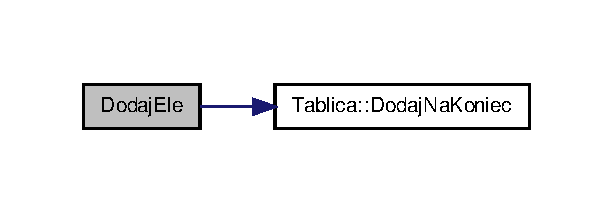
\includegraphics[width=294pt]{operacje_8hpp_a622767484b449600cf6446da085c561e_cgraph}
\end{center}
\end{figure}




Oto graf wywoływań tej funkcji\-:
\nopagebreak
\begin{figure}[H]
\begin{center}
\leavevmode
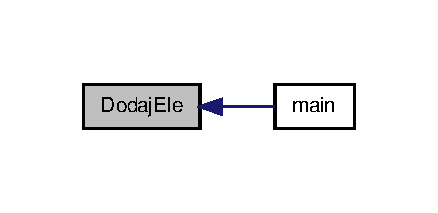
\includegraphics[width=210pt]{operacje_8hpp_a622767484b449600cf6446da085c561e_icgraph}
\end{center}
\end{figure}


\hypertarget{operacje_8hpp_afcebfcc0c075278505a19b1c9afff30d}{\index{operacje.\-hpp@{operacje.\-hpp}!Dodaj\-Ele@{Dodaj\-Ele}}
\index{Dodaj\-Ele@{Dodaj\-Ele}!operacje.hpp@{operacje.\-hpp}}
\subsubsection[{Dodaj\-Ele}]{\setlength{\rightskip}{0pt plus 5cm}void Dodaj\-Ele (
\begin{DoxyParamCaption}
\item[{{\bf Tablica} \&}]{T1, }
\item[{{\bf Tablica} \&}]{T2, }
\item[{double}]{ele}
\end{DoxyParamCaption}
)}}\label{operacje_8hpp_afcebfcc0c075278505a19b1c9afff30d}


Definicja w linii 20 pliku operacje.\-cpp.



Oto graf wywołań dla tej funkcji\-:
\nopagebreak
\begin{figure}[H]
\begin{center}
\leavevmode
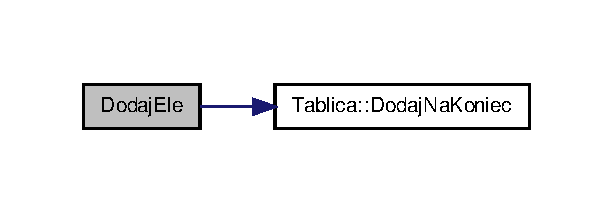
\includegraphics[width=294pt]{operacje_8hpp_afcebfcc0c075278505a19b1c9afff30d_cgraph}
\end{center}
\end{figure}


\hypertarget{operacje_8hpp_a0933bc7e6ecc1138cde73ad221d3a6a6}{\index{operacje.\-hpp@{operacje.\-hpp}!Odwroc\-Tab@{Odwroc\-Tab}}
\index{Odwroc\-Tab@{Odwroc\-Tab}!operacje.hpp@{operacje.\-hpp}}
\subsubsection[{Odwroc\-Tab}]{\setlength{\rightskip}{0pt plus 5cm}void Odwroc\-Tab (
\begin{DoxyParamCaption}
\item[{{\bf Tablica} \&}]{T}
\end{DoxyParamCaption}
)}}\label{operacje_8hpp_a0933bc7e6ecc1138cde73ad221d3a6a6}


Definicja w linii 9 pliku operacje.\-cpp.



Oto graf wywołań dla tej funkcji\-:
\nopagebreak
\begin{figure}[H]
\begin{center}
\leavevmode
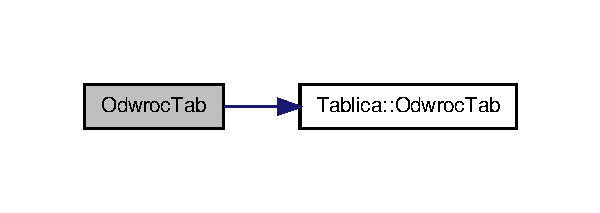
\includegraphics[width=288pt]{operacje_8hpp_a0933bc7e6ecc1138cde73ad221d3a6a6_cgraph}
\end{center}
\end{figure}




Oto graf wywoływań tej funkcji\-:
\nopagebreak
\begin{figure}[H]
\begin{center}
\leavevmode
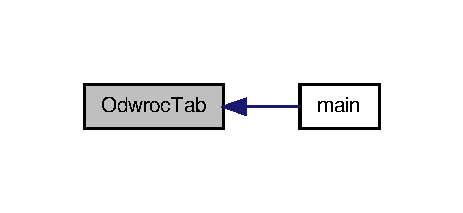
\includegraphics[width=222pt]{operacje_8hpp_a0933bc7e6ecc1138cde73ad221d3a6a6_icgraph}
\end{center}
\end{figure}


\hypertarget{operacje_8hpp_a0e1dcf6202da97bb49029fd97c1dc6a9}{\index{operacje.\-hpp@{operacje.\-hpp}!Zamien\-Ele@{Zamien\-Ele}}
\index{Zamien\-Ele@{Zamien\-Ele}!operacje.hpp@{operacje.\-hpp}}
\subsubsection[{Zamien\-Ele}]{\setlength{\rightskip}{0pt plus 5cm}void Zamien\-Ele (
\begin{DoxyParamCaption}
\item[{{\bf Tablica} \&}]{T, }
\item[{int}]{m1, }
\item[{int}]{m2}
\end{DoxyParamCaption}
)}}\label{operacje_8hpp_a0e1dcf6202da97bb49029fd97c1dc6a9}


Definicja w linii 4 pliku operacje.\-cpp.



Oto graf wywołań dla tej funkcji\-:
\nopagebreak
\begin{figure}[H]
\begin{center}
\leavevmode
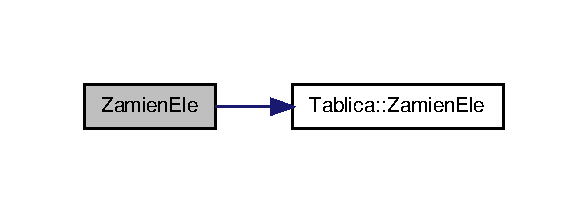
\includegraphics[width=282pt]{operacje_8hpp_a0e1dcf6202da97bb49029fd97c1dc6a9_cgraph}
\end{center}
\end{figure}




Oto graf wywoływań tej funkcji\-:
\nopagebreak
\begin{figure}[H]
\begin{center}
\leavevmode
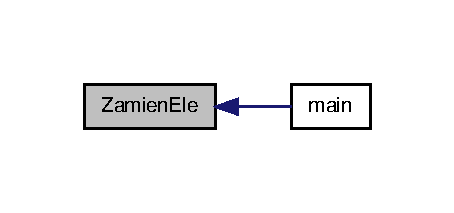
\includegraphics[width=218pt]{operacje_8hpp_a0e1dcf6202da97bb49029fd97c1dc6a9_icgraph}
\end{center}
\end{figure}



\hypertarget{tablica_8cpp}{\section{Dokumentacja pliku prj/tablica.cpp}
\label{tablica_8cpp}\index{prj/tablica.\-cpp@{prj/tablica.\-cpp}}
}


Definicja metody Dodaj\-Na\-Koniec.  


{\ttfamily \#include \char`\"{}tablica.\-hpp\char`\"{}}\\*
{\ttfamily \#include $<$fstream$>$}\\*
Wykres zależności załączania dla tablica.\-cpp\-:
\nopagebreak
\begin{figure}[H]
\begin{center}
\leavevmode
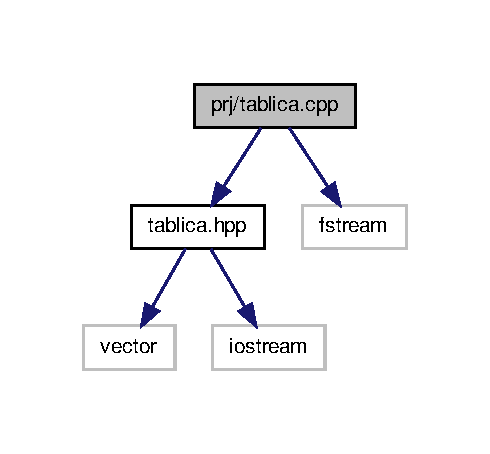
\includegraphics[width=235pt]{tablica_8cpp__incl}
\end{center}
\end{figure}


\subsection{Opis szczegółowy}
Definicja metody Dodaj\-Na\-Koniec. Definicja przeladowania operatora == .

Definicja przeladowania operatora = .

Definicja przeladowania operatora + .

Definicja metody Usun\-Ele.

Definicja metody Wyswietl\-Tab.

Definicja metody Pobierz\-Wskazany\-Ele.

Definicja metody Dodaj\-Na\-Miejsce.

Definicja metody Odwroc\-Tab.

Definicja metody zamien elementy.

Definicja metody Pobierz\-Rozmiar.

Definicja metody Pobierz\-Ostatni\-Ele.

Definicja metody Pobierz\-Pierwszy\-Ele.

Definicja metody Dodaj\-Na\-Poczatek.

Metoda, ktora dodaje na koniec element.

Metoda, ktora dodaje na poczatek element.

Metoda, ktora pobiera pierwszy element.

Metoda, ktora pobiera ostatni element.

Metoda, ktora pobiera pobiera rozmiar tablicy.

Metoda, ktora zamienia dwa wybrane elementy.

Metoda, ktora odwraca tablice.

Metoda, ktora dodaje element na konretne miejsce.

Metoda, ktora pobiera wskazany element.

Metoda, ktora wyswietla tabilce.

Metoda, ktora dusuwa elementy.

W celu lacznia dwoch tablic w jedna.

W celu przypisania dwoch tablic.

W celu lacznia porownania tablic. 

Definicja w pliku \hyperlink{tablica_8cpp_source}{tablica.\-cpp}.


\hypertarget{tablica_8hpp}{\section{Dokumentacja pliku C\-:/\-Users/\-Klijek/\-Desktop/\-L\-A\-B4/prj/tablica.hpp}
\label{tablica_8hpp}\index{C\-:/\-Users/\-Klijek/\-Desktop/\-L\-A\-B4/prj/tablica.\-hpp@{C\-:/\-Users/\-Klijek/\-Desktop/\-L\-A\-B4/prj/tablica.\-hpp}}
}


Definicja klasy \hyperlink{class_tablica}{Tablica}.  


{\ttfamily \#include $<$vector$>$}\\*
{\ttfamily \#include $<$iostream$>$}\\*
Wykres zależności załączania dla tablica.\-hpp\-:
Ten wykres pokazuje, które pliki bezpośrednio lub pośrednio załączają ten plik\-:
\subsection*{Komponenty}
\begin{DoxyCompactItemize}
\item 
class \hyperlink{class_tablica}{Tablica}
\end{DoxyCompactItemize}


\subsection{Opis szczegółowy}
Definicja klasy \hyperlink{class_tablica}{Tablica}. Klasa odpowiadaj�ca za operacje wykonujace sie na tablicy takie jak\-: zamienienie elementow, odwrocenie tablicy, dodanie elementu, dodanie elementow, operator + operator, operato == Oraz sortowania wykonywane dla stosu, a mianowicie quicksort, mergesort oraz heapsort. 

Definicja w pliku \hyperlink{tablica_8hpp_source}{tablica.\-hpp}.


\hypertarget{zegar_8cpp}{\section{Dokumentacja pliku prj/zegar.cpp}
\label{zegar_8cpp}\index{prj/zegar.\-cpp@{prj/zegar.\-cpp}}
}


Definicja metody Start.  


{\ttfamily \#include \char`\"{}zegar.\-hpp\char`\"{}}\\*
Wykres zależności załączania dla zegar.\-cpp\-:
\nopagebreak
\begin{figure}[H]
\begin{center}
\leavevmode
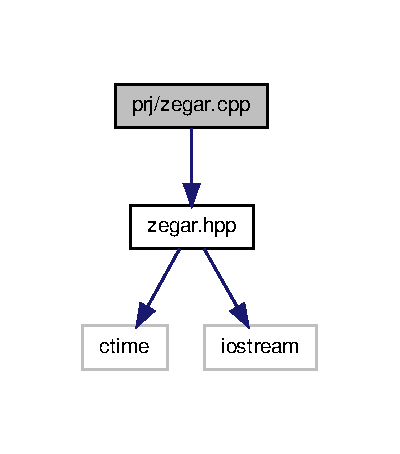
\includegraphics[width=192pt]{zegar_8cpp__incl}
\end{center}
\end{figure}


\subsection{Opis szczegółowy}
Definicja metody Start. Definicja metody Wynik.

Definicja metody Koniec.

Metoda, ktora powoduje start zegara.

Metoda, ktora powoduje stop zegara i oblicza czas.

Metoda, ktora wyswietla wynik. 

Definicja w pliku \hyperlink{zegar_8cpp_source}{zegar.\-cpp}.


\hypertarget{zegar_8hpp}{\section{Dokumentacja pliku prj/zegar.hpp}
\label{zegar_8hpp}\index{prj/zegar.\-hpp@{prj/zegar.\-hpp}}
}


Definicja klasy \hyperlink{class_tablica}{Tablica}.  


{\ttfamily \#include $<$ctime$>$}\\*
{\ttfamily \#include $<$iostream$>$}\\*
Wykres zależności załączania dla zegar.\-hpp\-:
\nopagebreak
\begin{figure}[H]
\begin{center}
\leavevmode
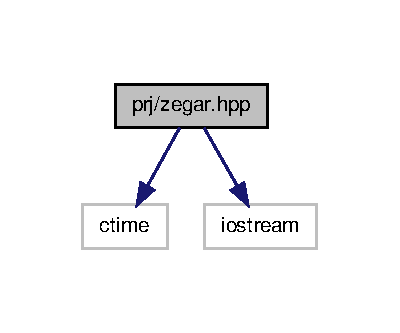
\includegraphics[width=192pt]{zegar_8hpp__incl}
\end{center}
\end{figure}
Ten wykres pokazuje, które pliki bezpośrednio lub pośrednio załączają ten plik\-:
\nopagebreak
\begin{figure}[H]
\begin{center}
\leavevmode
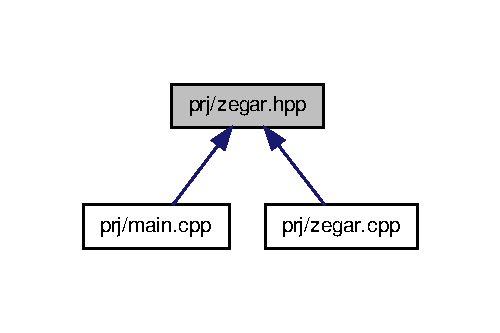
\includegraphics[width=240pt]{zegar_8hpp__dep__incl}
\end{center}
\end{figure}
\subsection*{Komponenty}
\begin{DoxyCompactItemize}
\item 
class \hyperlink{class_zegar}{Zegar}
\end{DoxyCompactItemize}


\subsection{Opis szczegółowy}
Definicja klasy \hyperlink{class_tablica}{Tablica}. Klasa odpowiadaj�ca za operacje wykonujace sie na tablicy takie jak\-: zamienienie elementow, odwrocenie tablicy, dodanie elementu, dodanie elementow, operator + operator, operato == 
\begin{DoxyParams}[1]{Parametry}
\mbox{\tt in}  & {\em clock\-\_\-t} & start, koniec -\/ zmienne przechowuja aktualny czas systemu \\
\hline
\mbox{\tt in}  & {\em czas} & -\/ przechowuje roznice czasow koniec i start \\
\hline
\end{DoxyParams}


Definicja w pliku \hyperlink{zegar_8hpp_source}{zegar.\-hpp}.


\printindex
\end{document}
